\documentclass[10pt]{article}
\usepackage{fullpage}
\usepackage{graphicx}
\usepackage{amssymb}
\usepackage{qtree}
\usepackage{rotating}
\newcommand{\tab}{\hspace*{2em}}
\newcommand{\tabb}{\hspace*{4em}}
\newcommand{\tabbb}{\hspace*{6em}}
\newcommand{\tabbbb}{\hspace*{8em}}
\newcommand{\tabbbbb}{\hspace*{10em}}
\newcommand{\norm}[1]{\left|\left|#1\right|\right|}
\setlength{\parindent}{0in} 
\begin{document}
	\begin{flushright}
	Lindsey Bieda and Joe Frambach\\
	Reduction and Parallel Problems\\
	10.31.2011
	\end{flushright}
	17. Consider the following problem. The input is an undirected graph $G$ and an integer $k$. The problem
	is to determine if $G$ contains a clique of size $k$ \textbf{AND} an independent set of size $k$. Recall that a
	clique is a collection of mutually adjacent vertices, and an independent set is a collection of mutually
	nonadjacent vertices. Show by reduction that if this problem has a polynomial time algorithm then
	the clique problem has a polynomial time algorithm.
	\\
	\\
	\textbf{CLIQUE} $\leq$ \textbf{CLIQUE\_AND\_INDSET}
	\\
	\\
	Program CLIQUE:\\
	\tab Read graph $G$, int $k$.\\
	\tab $G^\prime$ = $G$ + $k$ nodes not connected to any other nodes in $G$.\\
	\tab Return CLIQUE\_AND\_INDSET($G^\prime$,$k$).\\
	\\
	\\
	Since $G$ will contain an independent set of size $k$ as it is added to the original graph, CLIQUE\_AND\_INDSET 
	will always find an independent set of size $k$. The only aspect that is determined by the original input is if 
	there is a clique of size $k$, which is the desired functionality. 
	
	\newpage

	18. Consider the following problem. The input is an undirected graph $G$ and an integer $k$. The problem
	is to determine if $G$ contains a clique of size $k$ \textbf{OR} an independent set of size $k$. Show by reduction
	that if this problem has a polynomial time algorithm then the clique problem has a polynomial time
	algorithm.
	\\
	\\
	\textbf{CLIQUE} $\leq$ \textbf{CLIQUE\_OR\_INDSET}
	\\
	\\
	Program CLIQUE:\\
	\tab Read graph $G$, int $k$.\\
	\tab $G^\prime$ = $G$ + a new node connected to all other nodes in $G$.\\
	\tab Return CLIQUE\_OR\_INDSET($G^\prime$,$k + 1$).\\

		\begin{figure}[h]
		\centering
		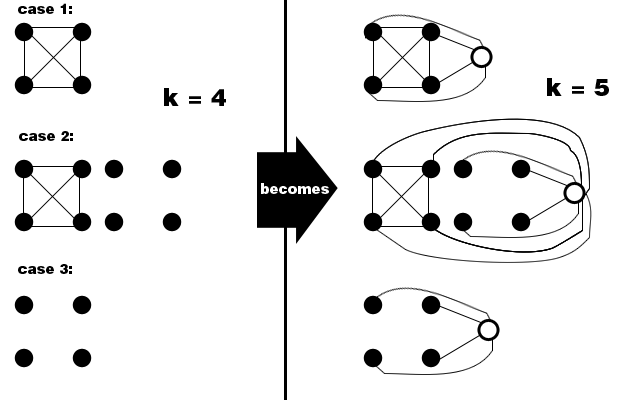
\includegraphics[width=290px]{cliqueoris.png}
		\caption{Construction of $G^\prime$}
		\end{figure}
		
	Figure 1 shows how the construction of the new $G^\prime$ and by increasing the value of $k$ we ensure that
	CLIQUE\_OR\_INDSET($G^\prime$,$k + 1$) will return true, if and only if $G$ contains a clique of size $k$. 
	This is the case since we eliminate the independent set by adding the new node and increase the size of the 
	possibly existing clique with the addition of this new node.
	
	\newpage


	22. Consider the following problem. The input is a graph $G = (V, E)$, a subset $R$ of vertices of $G$, and a
	positive integer $k$. The problem is to determine if there is a subset $U$ of $V$ such that
	\begin{enumerate}
		\item All the vertices in $R$ are contained in $U$, and
		\item the number of vertices in $U$ is at most $k$, and
		\item for every pair of vertices $x$ and $y$ in $R$, one can walk from $x$ to $y$ in $G$ only traversing vertices that
		are in $U$.
	\end{enumerate}
	Show that this problem is NP-hard using a reduction from Vertex Cover. Recall that the input for the
	vertex cover problem is a graph $H$ and an integer $\ell$, and the problem is to determine whether $H$ has a
	vertex cover of size $\ell$ or not. A vertex cover $S$ is a collection of vertices with the property that every
	edge is incident on at least one vertex in $S$.

	\newpage

	1. Consider the problem of computing the AND of $n$ bits.
	\begin{itemize}
		\item Give an algorithm that runs in time O(log $n$) using n processors on an EREW PRAM. What is
		the efficiency of this algorithm?\\
		\\
		The parallel algorithm works as follows:\\
		AND($x_1, \ldots, x_n$, $p$)\\
		If $p$ = 1:\\
		\tab $p$ returns the value it has\\
		Else:\\
		\tab and(AND($x_1, \ldots, x_{n/2}$, $p/2$), AND($x_{n/2 + 1}, \ldots, x_n$, $p/2$)), where lowercase 
		and refers to performing the and of the two returned values. 
		\begin{figure}[h]
		\centering
		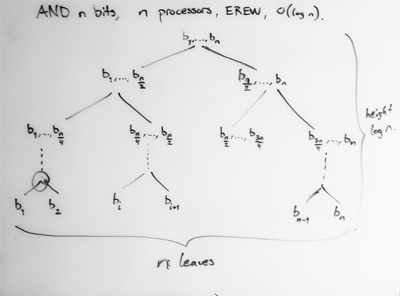
\includegraphics[width=290px]{parallel1.png}
		\caption{Construction of the tree}
		\end{figure}
		
		We end up with the above call tree which demonstrates that this algorithm performs in O(log $n$) time.\\
		The efficiency is: $n / (2n - 1)$
		
		\item Give an algorithm that runs in time O(log $n$) using $n/$log $n$ processors on an EREW PRAM.
		What is the efficiency of this algorithm?\\
		\\
		The parallel algorithm works as follows:\\
		AND($x_1, \ldots, x_n$, $p$)\\
		If $p$ = 1:\\
		\tab $p$ performs the following:\\
		\tabb For each bit:\\
		\tabbb if bit = 0: return 0\\
		\tabb return 1\\
		Else:\\
		\tab and(AND($x_1, \ldots, x_{n/2}$, $p/2$), AND($x_{n/2 + 1}, \ldots, x_n$, $p/2$)), where lowercase 
		and refers to performing the and of the two returned values.\\
		\\
		The tree structure is very similar to the one above, however, the height is now log(log $n$) and there are $n/($log$n)$ leaves.
		Each leaf takes log($n$) time to process the data.
		\\
		The efficiency is: $n/ ( n + (n/$log$ n ) - 1)$\\
		\\
		\item Give an algorithm that runs in time O(1) using n processors on a CRCW PRAM.\\
		\\
		Answer = 1\\
		\\
		For processor $i = 1$ to $n$:\\
		\tab $processor_i$ runs:\\
		\tabb If $b_i$ == 0:\\
		\tabbb Anwser = 0.\\
		return Answer.\\
		\\
		Each processor takes one bit and if it is a 0 they write a 0 to the answer memory location.  
	\end{enumerate}
\end{document}
